\documentclass[border=8pt]{standalone}
\usepackage{tikz}
\usetikzlibrary{arrows.meta,positioning,backgrounds,fit}

%  dissertation palette anchored on red rgb(0.549,0.176,0.098) = #8C2D18 
\definecolor{redFill}{HTML}{F5E8E4}   % critique boxes, loop enclosure bg
\definecolor{redLine}{HTML}{8C2D18}   % = engineering anchor color
\definecolor{redText}{HTML}{3A1009}
\definecolor{slateFill}{HTML}{EAEDF0} % draft / member boxes
\definecolor{slateLine}{HTML}{6B7E8C}
\definecolor{slateText}{HTML}{2E404D}
\definecolor{sandFill}{HTML}{FAF5EE}  % final / consensus / Borda
\definecolor{sandLine}{HTML}{B8A070}
\definecolor{sandText}{HTML}{5A4118}
\definecolor{tealFill}{HTML}{E5F0ED}  % rewrite / positive action
\definecolor{tealLine}{HTML}{3D7A6A}
\definecolor{tealText}{HTML}{1E4D41}
\definecolor{arrowGray}{HTML}{8A8880} % flow arrows, phase labels
\definecolor{phaseText}{HTML}{3D3C38}

\begin{document}
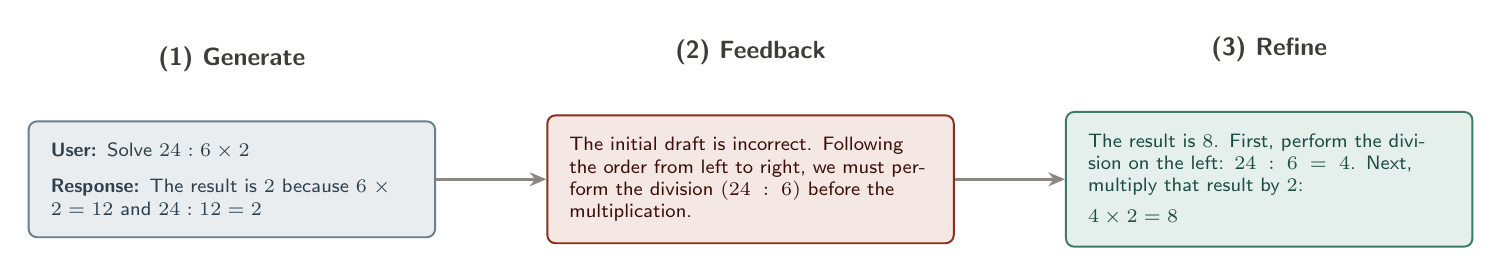
\begin{tikzpicture}[
  font=\sffamily,
  phase/.style={font=\sffamily\bfseries\small, text=phaseText},
  box/.style={
    rectangle, rounded corners=3pt,
    draw, line width=0.7pt,
    text width=46mm, align=left,
    inner sep=8pt, font=\sffamily\scriptsize
  },
  slatebox/.style={box, fill=slateFill, draw=slateLine, text=slateText},
  redbox/.style={box, fill=redFill, draw=redLine, text=redText},
  tealbox/.style={box, fill=tealFill, draw=tealLine, text=tealText},
  flow/.style={-{Stealth[length=6pt,width=5pt]}, line width=1.1pt, draw=arrowGray}
]

%  Stage boxes 
\node[slatebox] (gen) {%
  \textbf{User:} Solve $24 : 6 \times 2$
  \par\vspace{5pt}
  \textbf{Response:} The result is $2$ because $6\times2=12$ and $24:12=2$
};

\node[redbox, right=14mm of gen] (fb) {%
  The initial draft is incorrect. Following the order from left to right, we must perform the division $(24:6)$ before the multiplication.
};

\node[tealbox, right=14mm of fb] (ref) {%
  The result is $8$. First, perform the division on the left: $24:6=4$. Next, multiply that result by $2$:
  \par\vspace{3pt}
  $4 \times 2 = 8$
};

%  Phase labels 
\node[phase, above=5mm of gen] {(1) Generate};
\node[phase, above=5mm of fb]  {(2) Feedback};
\node[phase, above=5mm of ref] {(3) Refine};

%  Flow arrows 
\draw[flow] (gen) -- (fb);
\draw[flow] (fb)  -- (ref);

\end{tikzpicture}
\end{document}